\begin{center}
    \chapter{Uzdevumi}
\end{center}

\section{Uzdevumu izvēles pamatojums}

Praktiskai saskarņu salīdzināšanai nepieciešams definēt programmēju problēmu,
kuru iespējams izstrādāt uz visām platformām.  Jāizvēlas tāds uzdevums, kuru
iespējams 'augsti' paralelizēt, tas ir, sadalīt uzdevumu daudzos mazos un (it
īpaši) neatkarīgos gabalos, lai būtu pievienotā vērtība (ātrdarbība) to pildīt
uz GPU, ņemot vērā papildus darbu un nepieciešamās zināšanas, lai ieviestu GPU
risinājumu.

Tā kā uzdevuma risinājumu primārais mērķis ir izmantot etalonuzdevumā, tad
tam ir jābūt tādam, ar kuru iespējams notestēt kādu biežu lietotu GPGPU
platformu funkciju apakškopu.

Viena uzdevuma ietvaros varētu rasties šaubas par etalonuzdevuma rezultātu
ticamību, tas ir, iespējams radītie risinājumi, uzstādījums vai pats uzdevums
radījis kādu īpašu situāciju, kurā kāda konkrēta platforma noteiktos mērījumos
izvirzās vadībā, kas nebūtu tiesa citās reālās programmās ar pievienoto
vērtību. Tāpēc tiek izvirzīta prasība pēc diviem dažādiem uzdevumiem.

Par vienu uzdevumu tiks izmantots jau autora kursa darbā definētais un 
izstrādatais uzdevums (uz CUDA un ROCm, bet ne OpenCL) - paroļu lauzējs,
atguvējs priekš SHA-256 jauktām, šifrētām parolēm.\cite{kursa-darbs}

Nobriedušāki paroļi lauzēji, jeb precīzāk - paroļu atkopēji kā
"hashcat"\cite{hashcat} ir spējīgi ņemt vērā vairākas paroļu variācijas,
maskas, faktus, ka parole, piemēram, iesākusies ar "123" un citas sarežģītākas
potenciālo paroļu iegūšanas metodes. Demonstrācijas vajadzībām pietiktu
izstrādāt pašu 'kodolu', kas, ar jau saņemtu iespējamo paroļu sarakstu, tās
pārbaudīs, jeb tā sauktais 'vārdnīcas' tipa uzbrukums.\cite{hashcat_dict_atk}

Šādā uzdevuma implementācijās būs nepieciešamība izmantot datu straumi parolēm,
pie atbilstošas paroles atrašanas, jānodrošina atomiska datu ierakstīšana no
attiecīgā veiksmīgā GPGPU pavediena. Kā arī šim uzdevumam, ņemot vērā definētu
straumes bufera izmēru un apstrādājamo paroļu skaitu, ir fiksēts izpildāmo
GPGPU kodolu un laidienu skaits. Daudzos praktiskos scenārijos GPU resursi tiek
izmantoti ilgtermiņa darbībām, kur izpildāmo kodolu skaits varētu nebūt
definēts, piemēram, mākslīgā intelekta mašīnmācīšanās modeļi, kuri tiek trenēti
kamēr sasniegts kāds kvalitātes kritērijs.

Noteiktajos etalonuzdevuma prasību ietvaros tomēr vajadzētu kādu statiski
nosakāmu izpildes apjomu, tāpēc, lai notestētu šādu ilgtermiņa izpildi tiek
noteikts otrs uzdevums - Džona Konveja dzīves spēles \cite{conway1970conway}
realizācija, kurā izpildes apjoms definējams kā šūnu automāta darbības soļi.

Šīs šūnu automāts ir viens no zināmākajiem tā vienkāršo noteikumu un
iespējamās kompleksās šūnu mijiedarbības dēļ (ar to iespējams
uzkonstruēt jebkuru Tjūringa mašīnu). Šūnas ir izkārtotas 2 dimensionālā režģī,
virmsā. Katra šūna ir vai nu dzīva vai mirusi un nākamajā solī šūnas stāvoklis
ir atkarīgs no tās tiešajiem 8 kaimiņiem\cite{conway1970conway}:
\begin{itemize}
    \item ja šūna ir mirusi:
        \begin{itemize}
            \item ja tai ir precīzi 3 kaimiņi, tā nākamajā solī būs dzīva,
            \item jebkurā citā situācijā tā paliks mirusi.
        \end{itemize}
    \item ja šūna ir dzīva:
        \begin{itemize}
            \item ja tai ir 2 vai trīs kaimiņi, tā paliks dzīva,
            \item ja tai vai nu mazāk par 2 vai vairāk par 3 kaimiņiem,
                tā nākamajā solī nomirs (it kā vai nu no nepietiekamas
                apdzīvotības vai pārapdzīvotības).
        \end{itemize}
\end{itemize}

Uzdevumu ir vērts pildīt uz GPU, jo katru automāta šūnu iespējams apstrādāt
savā pavedienā gandrīz vai kā 2D bildi, kur katrs pikselis atbilst katrai
automāta šūnai. Papildus sarežģītība un iespējamās platformu ātrdarbības
atšķirības meklējamas GPU atmiņas datu izveidē un apmaiņā pie liela spēles soļu
skaita, jo ar katru soli nākas mainīt ieejas datus, izejas datus.


\section{Programmatūras, aparatūras uzstādījums}
Tā kā programmas notikumu ilgumi dažādās konfigurācijās nāks no CPU, CUDA, HIP
un OpenCL pusēm, tad lai būtu vienota un viegli apstrādājama datu kopa,
notikumi tiks žurnalēti failā, izmantojot, spdlog\cite{spdlog-github}, C++
žurnalēšanas bibliotēku.

Ērtai datu apstrādei, izmantojamais faila formāts ir CSV, un datu formāts
skatāms izdrukā \ref{lst:benchmark_log_example}.

\begin{lstlisting}[caption={Etalonuzdevuma žurnālfaila ieraksta formāts},
  label=lst:benchmark_log_example,
  captionpos=t
]
<Platformas tips>,<Notikuma apraksts>,<Ilgums, ms>
OpenCL, Kodola izpildes laiks, 2.0736
CUDA, Datu parraide uz GPU, 1.83927
HIP, Atminas malloc uz GPU, 6.42058
\end{lstlisting}

Notikuma ilgums norādāms milisekundēs, jo, galvenokārt, tādā mērvienībā
notikumu ilgumu noklusēti atgriež gan CUDA, gan HIP profilēšanas funkcijas
\textit{cudaEventElapsedTime}, \textit{hipEventElapsedTime}. OpenCL funkcija
\textit{clGetEventProfilingInfo} atgriež notikuma ilgumu nanosekundēs, šajā
gadījumā rezultāti tiks pārveidoti, lai nodrošinātu konsekvenci starp pārējām
platformām.

Uzdevumu izstrādei, testēšanai un etalonuzdevumu izpildei izmantots dators ar:
\begin{itemize}
    \item Arch Linux operētājsistēmu ar Linux 6.14.5-arch1-1 OS kodolu
    \item AMD Ryzen 5600H procesoru ar Radeon Graphics integrēto videokarti,
    \item Nvidia GeForce RTX 3060 Laptop ārējo videokarti.
\end{itemize}

Lai nodrošinātu risinājumu izolāciju caur Docker, visu konteineru izveidē par
bāzes Docker bildi izmantota Ubuntu 24.04. Par pamata Docker failu HIP
risinājumam izmantots AMD izstrādatais \cite{amd_dockerfile} ar sagatavotu vidi
ROCm un CUDA platformām. Līdzīgi priekš CUDA izmantota Nvidia
sagatavotā bilde\cite{nvidia_dockerfile}, kurai pamatā ir Ubuntu (pilnās Docker bilžu
atkarības skatīt attēlā \ref{fig:directed-graph}).

\begin{figure}[h]
  \centering
  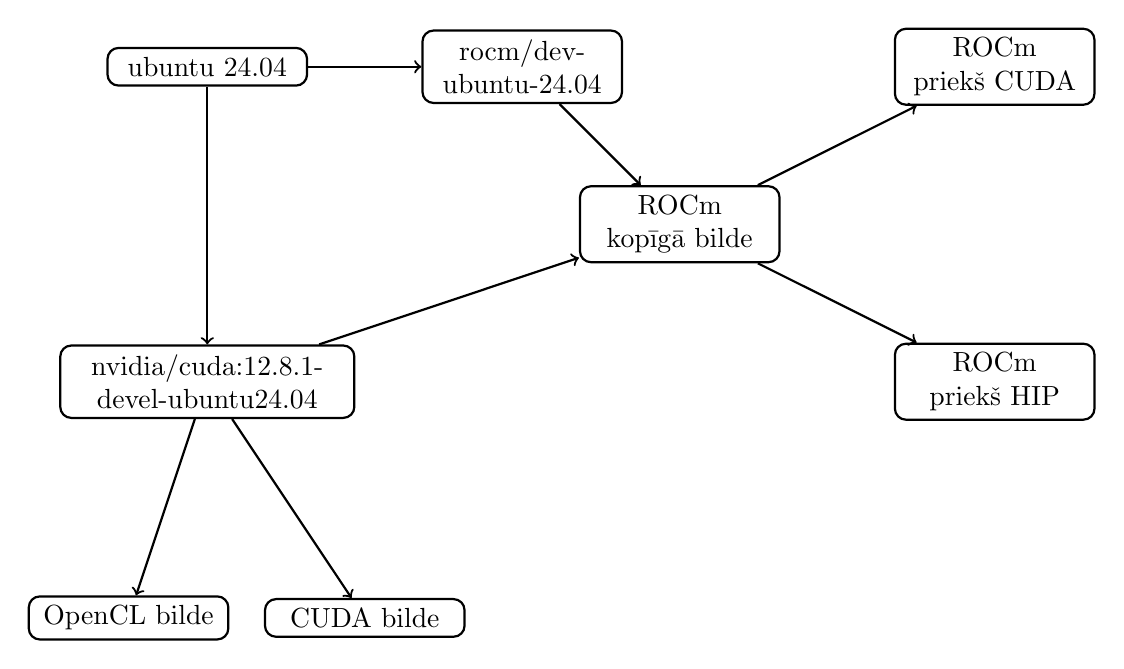
\begin{tikzpicture}
    \node[draw, rounded corners, thick, minimum width=2.5cm, text width=2.3cm, align=center] (1) at (0,4) {ubuntu 24.04};
    \node[draw, rounded corners, thick, minimum width=2.5cm, text width=3.5cm, align=center] (2) at (0,0) {nvidia/cuda:12.8.1-devel-ubuntu24.04};
    \node[draw, rounded corners, thick, minimum width=2.5cm, text width=2.3cm, align=center] (3) at (4,4) {rocm/dev-ubuntu-24.04};
    \node[draw, rounded corners, thick, minimum width=2.5cm, text width=2.3cm, align=center] (4) at (6,2) {ROCm kopīgā bilde};
    \node[draw, rounded corners, thick, minimum width=2.5cm, text width=2.3cm, align=center] (5) at (10,4) {ROCm priekš CUDA};
    \node[draw, rounded corners, thick, minimum width=2.5cm, text width=2.3cm, align=center] (6) at (10,0) {ROCm priekš HIP};
    \node[draw, rounded corners, thick, minimum width=2.5cm, text width=2.3cm, align=center] (7) at (2,-3) {CUDA bilde};
    \node[draw, rounded corners, thick, minimum width=2.5cm, text width=2.3cm, align=center] (8) at (-1,-3) {OpenCL bilde};
    
    \draw[->, thick] (1) -- (3);
    \draw[->, thick] (1) -- (2);
    \draw[->, thick] (2) -- (7);
    \draw[->, thick] (2) -- (8);
    \draw[->, thick] (2) -- (4);
    \draw[->, thick] (3) -- (4);
    \draw[->, thick] (4) -- (5);
    \draw[->, thick] (4) -- (6);
  \end{tikzpicture}
  \caption{Docker pamatbilžu atkarības}
  \label{fig:directed-graph}
\end{figure}

Pašu programmu izstrādei un kompilēšanai izmantots sekojošs programmatūras
steks ar fiksētām versijām:

\begin{itemize}
    \item Make 4.4.1-2
    \item CMake 4.0.1-2
    \item gcc 15.1.1
    \item CUDA, nvcc 12.8.97
    \item ROCm HIP, hipcc 6.3.4
    \item spdlog 1.15.2-1
\end{itemize}

\section{Paroļu atguvēja īstenojums} \label{sha256_section}
Tātad jāizstrādā programma, kura, ņemot vērā ieejas failu ar potenciālajām
parolēm, no kādas paroles jaucējvērtības spētu noskaidrot pašu paroli. Uzdevumu
būtu vērts risināt uz GPU, jo pie liela paroļu skaita, katrs GPU pavediens
neatkarīgi no citiem varētu rēķināt savas paroles jaucējvērtību un pārbaudīt to
pret uzlaužamo.

Programma ir paredzēta kā komandrindas utilīta ar CLI argumentiem:
\begin{itemize}
    \item ievades faila ceļš,
    \item paroles jaucējvērtība,
    \item žurnālfaila ceļs
\end{itemize}

Apstrādājamais fails saturēs potenciālās paroles (piemēru skatīt izdrukā
\ref{lst:pw_file_example}, katra savā rindā, kurām tiks izrēķināta
jaucējvērtība un salīdzināta pret doto. Izmantojamais jaukšanas algoritms -
SHA256. Jaucējvērtību rēķināšana un salīdzināšana jārealizē izpildei uz GPU.
\cite{kursa-darbs}

\begin{lstlisting}[caption={Paroļu ieejas faila piemērs ar nejauši ģenerētām parolēm}, label=lst:pw_file_example]
5QW8ZywwXSQ8I
YIqBz6PgEbDg3AK
qs0xxkco3AYaX
zRX5l1
qyGgl8Dg
cvJTiLCw7e
ySBinJCvd
7cDTl7RsdLFhD
...
\end{lstlisting}

SHA256 izvēlēts tā tīri tā popularitātes un relatīvi ātrās izpildes dēļ,
paroles uzlaušanas demonstrācijas vajadzībām ar šo pietiek, nepieciešamības
gadījumā iespējams ieviest citu jaukšanas algoritmu un aizstāt ar esošo.

Lai notestētu SHA-256 aprēķinu darbību pret zināmām jaucējvērtībām un to
attiecīgajiem ziņojumiem, kā arī, lai pārbaudītu vispārīgu GPGPU kodola
programmas darbību, platformas pieejamību uz šī datora apartūras, un veiktu
galveno programmas izpildes, programma jādarbina no komandrinas, padodot
atbilstošos argumentus (skatīt izdruku  \ref{lst:pwcracker_mains}). \cite{kursa-darbs}

\begin{lstlisting}[caption={Programmas galvenā izpilde}, label=lst:pwcracker_mains]
$ pwcracker <parolu faila cels> <paroles hash vertiba> <zurnalfaila cels>
\end{lstlisting}

Algoritmu skatīt izdrukās \ref{lst:sha256_pseido_alg}.
\begin{lstlisting}[caption={Paroļu atguvēja CPU puses pseidokods}, label=lst:sha256_pseido_alg]
passwords, offsets, count =  readPasswordFromFile(inputFile)
log(fileLoadTime())

passwordsPinnedMemory = mallocPinnedMemory(sizeof(passwords))
offsetsPinnedMemory = mallocPinnedMemory(sizeof(of\cite{amd_dockerfile}fsets))

devicePasswordsBuffer = deviceMalloc(sizeof(passwords))
deviceOffsetsBuffer = deviceMalloc(sizeof(offsets))
deviceHash = deviceMalloc(sizeof(32)) // sha 256 biti => 32 baiti
deviceOutputIdx = deviceMalloc(sizeof(4)) // int izmers ieks C/C++
log(bufferCreationTime())

hostMemcpy(passwordsPinnedMemory, passwords)
hostMemcpy(offsetsPinnedMemory, offsets)
deviceMemcpy(devicePasswordsBuffer, passwordsPinnedMemory)
deviceMemcpy(deviceOffsetsBuffer, offsetsPinnedMemory)
deviceMemcpy(deviceHash, hash)
deviceMemcpy(deviceOutputIdx, -1)
log(hostToDeviceMemoryTransferTime())


PwCracker(devicePasswordsBuffer, deviceOffsetsBuffer, passwords.count(), deviceHash, deviceOutputIdx)
log(kernelExecTime())

if outputIdx != -1
    print(passwords[outputIdx])
\end{lstlisting}


\begin{lstlisting}[caption={Paroļu atguvēja GPGPU kodola pseidokods}, label=lst:sha256_pseido_alg_device]
PwCracker(passwords, pwOffsets, count, hash, outputIdx):
    i = blockIdx.x * blockDim.x + threadIdx.x

    password = passwords + pwOffsets[i]
    if i >= pwCount:
        return

    if sha256(password) == hash:
        atomicStore(outputIdx, i)
\end{lstlisting}

\section{Dzīves spēles šūnu automāta īstenojums} \label{gol_section}

Tāpat kā paroļu atguvējam, programma darbināma no komandrindas, padodot CLI
argumentus:
\begin{itemize}
    \item ievades režģa faila ceļš,
    \item izejas režģa faila ceļš,
    \item šūnu automāta izpildāmo soļu skaits,
    \item žurnālfaila ceļs. (skatīt izdruku \ref{lst:gol_mains}).
\end{itemize}

\begin{lstlisting}[caption={Programmas galvenā izpilde}, label=lst:gol_mains]
$ gol <ieejas rezga faila cels> <izejas rezga faila cels> <automata solu skaits> <zurnalfaila cels> 
\end{lstlisting}

Ieejas un izejas režģu failiem jāsastāv no vieniniekiem un nullēm,
reprezentējot faktu vai attiecīgā šūna ir dzīva (1) vai mirusi (0), izdruka
\ref{lst:gol_file_examples}.

\begin{lstlisting}[caption={Ieejas, izejas faila piemērs (ar tā saukto planiera rakstu)}, label=lst:gol_file_examples]
// ieejas fails:
0000000
0001000
0000100
0011100
0000000

// izejas fails pec viena sola:
0000000
0000000
0010100
0001100
0001000
\end{lstlisting}

Algoritma pseidokodu skatīt izdrukās \ref{lst:gol_pseido_alg} un  \ref{lst:gol_pseido_alg_device}.
\begin{lstlisting}[caption={Dzīves spēles šūnu automāta CPU puses pseidokods}, label=lst:gol_pseido_alg]
data, width, height = readGridFromFile(inputFile)
log(gridReadTime())

inputGridPinnedMemory = mallocPinnedMemory(sizeof(data))
outputGridPinnedMemory = mallocPinnedMemory(sizeof(data))

deviceInputBuffer = deviceMalloc(sizeof(data))
deviceOutputBuffer = deviceMalloc(sizeof(data))
log(bufferCreationTime())

hostMemcpy(inputGridPinnedMemory, data)
deviceMemcpy(deviceInputBuffer, inputGridPinnedMemory)
log(hostToDeviceMemoryTransferTime())

for i in range(0, gameSteps):
    GameOfLife(deviceInputBuffer, deviceOutputBuffer, width, height)
    log(kernelExecTime())

    swap(deviceInputBuffer, deviceOutputBuffer)

deviceMemcpyToHost(outputGridPinnedMemory, deviceInputBuffer)
log(deviceToHostMemoryTransferTime())

writeGridToFile(outputGridPinnedMemory, outputFile)
log(gridWriteTime())
\end{lstlisting}

\begin{lstlisting}[caption={Dzīves spēles šūnu automāta GPGPU kodola pseidokods}, label=lst:gol_pseido_alg_device]
GameOfLife(inputGrid, outputGrid, width, height):
    x = blockIdx.x * blockDim.x + threadIdx.x
    y = blockIdx.y * blockDim.y + threadIdx.y

    if x >= width || y >= height:
        return

    neighbors = neighborCount(inputGrid[y][x])
    
    cell = 0

    if input[y][x] == 1:
		if neighbors == 2 || neighbors == 3:
		    cell = 1
	else if neighbors == 3:
        ncell = 1;

    outputGrid[y][x] = cell
\end{lstlisting}

\section{Risinājumu kopējie ierobežojumi un skaidrojumi}
Abu programmu pseidokodi rakstīti pēc iespējas platform-neatkarīgi, bet, lai
būtu lielāka skaidrība par implementācijas detaļām, tabulā
\ref{tab:pseudocode_representations} minētas atbilstošās CUDA, HIP, OpenCL
funkcijas.

\begin{table}[h!]
\caption{Pseidokodā minēto funkciju atbilstošās funkcijas katrā platformā}
\label{tab:pseudocode_representations} 
\begin{tabularx}{\textwidth}{
  >{\raggedright\arraybackslash}p{0.225\textwidth}
  >{\raggedright\arraybackslash}p{0.16\textwidth}
  >{\raggedright\arraybackslash}p{0.15\textwidth}
  >{\raggedright\arraybackslash}p{0.365\textwidth}
}
\hline
\textbf{Pseidokoda funkcija} & \textbf{CUDA} & \textbf{ROCm HIP} & \textbf{OpenCL} \\ \hline
mallocPinnedMemory & cudaMallocHost & hipHostMalloc & clCreateBuffer ar CL\_MEM\_READ\_WRITE, CL\_MEM\_ALLOC\_HOST\_PTR karogiem \\ \hline
hostMemcpy & std::memcpy & std::memcpy & std::memcpy \\ \hline
deviceMalloc & cudaMalloc & hipMalloc & clCreateBuffer ar CL\_MEM\_READ\_WRITE karogu \\ \hline
deviceMemcpy & cudaMemcpy & hipMemcpy & clEnqueueWriteBuffer \\
\hline
\end{tabularx}
\end{table}

Mērāmie notikumu ilgumi kā pseidokodā norādīts ar, piemēram,
\textit{bufferCreationTime}, \textit{deviceToHostMemoryTransferTime} u. tml.,
realizējami ar prioritāri attiecīgajām GPGPU API notikumu profilēšanas
funkcijām, ja kādā vai visās kādu notikumu nav iespējams izmērīt, vai tas
neskaitās kā notikums, tad lietojama C++ standarta bibliotēkas datumu un laiku
manipulācijas bibliotēka "chrono".\cite{std_chrono}

\begin{lstlisting}[caption={"chrono" laika mērīšanas piemērs},
    label=lst:chrono_example]
auto start = std::chrono::steady_clock::now();
// meramais koda gabals
auto end = std::chrono::steady_clock::now();

std::chrono::duration<double, std::milli> elapsedTime = end - start;
\end{lstlisting}

\begin{lstlisting}[caption={CUDA laika mērīšanas piemērs},
    label=lst:cuda_example]
cudaEvent_t start, stop;
cudaEventCreate(&start);
cudaEventCreate(&stop);

cudaEventRecord(start);
// CUDA API izsaukumi
cudaEventRecord(stop);

float elapsedTime = 0;
cudaEventElapsedTime(&elapsedTime, start, stop);
\end{lstlisting}

\begin{lstlisting}[caption={ROCm HIP laika mērīšanas piemērs},
    label=lst:hip_example]
hipEvent_t start, stop;
hipEventCreate(&start);
hipEventCreate(&stop);

hipEventRecord(start);
// HIP API izsaukumi
hipEventRecord(stop);

float elapsedTime = 0;
hipEventElapsedTime(&elapsedTime, start, end);
\end{lstlisting}

\begin{lstlisting}[caption={OpenCL laika mērīšanas piemērs},
    label=lst:cl_example]
cl_event event;

clResult = clEnqueueNDRangeKernel(kernel, 1, nullptr, globalSize, localSize, 0, nullptr,

clFunkcijaKuraSanemCl_EventParametru(/*...*/, &event);

cl_ulong start;
cl_ulong end;

clGetEventProfilingInfo(event, CL_PROFILING_COMMAND_START, sizeof(start), &start, nullptr);
clGetEventProfilingInfo(event, CL_PROFILING_COMMAND_COMPLETE, sizeof(end), &end, nullptr);

float elapsedTime = static_cast<double>(end - start);
\end{lstlisting}

\section{Ievaddatu ģenerēšana un etalonuzdevuma darbināšana}
\subsection{Ģenerēšanas}
Paroļu atguvēja programmām, lai iegūtu nepieciešamos paroļu failus, izmantots
Python skripts\cite{kursa-darbs}, kas:
\begin{itemize}
    \item Nejauši ģenerē paroles pēc lietotāja ievadītā paroļu skaita,
    \item Katra parole ir garumā 6 - 16 un sastāv no ASCII simboliem.
\end{itemize}

Izvēlētas šādas prasības, jo paroles pārsvarā tiek definētas, izmantojot ASCII
simbolus, un tās  tiek rakstītas dotajā simbolu diapazonā.
\cite{pw_user_practice}

Skripts darbināms caur komandrindu, padodot CLI argumentus paroļu skaitam
un faila nosaukumam, ceļam (skatīt izdruku \ref{lst:pwgen_cli}).
\begin{lstlisting}[caption={Paroļu faila ģenerēšanas skripta darbināšana},
    label=lst:pwgen_cli, language=bash]
$ python3 ./pwgen.py <parolu skaits> <izejas faila cels>
\end{lstlisting}

Līdzīgi izveidots Dzīves spēles režģa ievadfaila ģenerēšanas skripts, kurš
katru šūnu nejauši aizpilda ar 1 vai 0. Skripts darbināms caur komandrindu,
padodot CLI arguments režģa platumam un garumam, faila nosaukumam (skatīt
izdruku \ref{lst:gridgen_cli}).

\begin{lstlisting}[caption={Režģa failaģenerēšanas skripta darbināšana},
    label=lst:gridgen_cli, language=bash]
$ python3 ./gridfile_gen.py <platums jeb x> <garums jeb y> <izejas faila cels>
\end{lstlisting}

\subsection{Etalonuzdevumu skripts}
Ņemot vērā izveidotās programmas un etalonuzdevumu izveides apsvērumus,
definētās katra uzdevuma risinājuma dažādas laidienu konfigurācijas.

Paroļu atguvējam noteikti sekojoši parametri: \cite{kursa-darbs}
\begin{itemize}
    \item Risinājuma platforma:
    \begin{itemize}
        \item CUDA 
        \item HIP 
        \item OpenCL 
    \end{itemize}
    \item Paroļu apjoms failā:
    \begin{itemize}
        \item 10 000 paroles
        \item 1 miljons paroles
        \item 100 miljonu paroļu
    \end{itemize}
    \item Laušanas rezultāts:
    \begin{itemize}
        \item Veikmsīgi atrasta parole
        \item Neatrasta parole
    \end{itemize}
    \item Uzlaužamās paroles atrašanās vieta failā:
    \begin{itemize}
        \item 1. kvartile (pirmie 25\%)
        \item 2. kvartile
        \item 3. kvartile
        \item 4. kvartile
    \end{itemize}
\end{itemize}


Tā kā tiek lietota ievaddatu straumēšana, tomēr kaut kādā apmērā notiek secīga
elementu apstrāde, dati tiek ielasīti un izņemti no GPU atmiņas, un kodoli
laisti pēc kārtas. Līdz ar to izpildes ilgums pie lieliem failu izmēriem ir
atkarīgs no paroļu skaita. Lai redzētu šo ietekmi un atšķirības starp
platformām, noteikta laidiena konfigurācija ar dažādiem paroļu garumiem un
paroles atrašanos failā, tās pozīciju.

Līdzīgi definēta Dzīves spēles laidiena konfigurācija:
\begin{itemize}
    \item Risinājuma platforma:
    \begin{itemize}
        \item CUDA 
        \item HIP 
        \item OpenCL 
    \end{itemize}
    \item Ieejas režģa izmērs
    \begin{itemize}
        \item 100x100 
        \item 1000x1000 
        \item 10000x10000
    \end{itemize}
    \item Automāta soļu skaits:
    \begin{itemize}
        \item 1 
        \item 100 
        \item 1000
        \item 10000
    \end{itemize}
\end{itemize}

Viena no etalonuzdevumu prasībām ir lieki nenoslogota sistēma, tāpēc, lai
etalonuzdevuma skripts mazinātu savu ietekmi uz sistēmu un attiecīgi
pēc iespējas mazāk ietekmētu programmas, mērķtiecīgi tiek iegūti visi
iespējamie dati darbam pirmsapstrādes solī, kurš beidzas ar piespiedu kārtā 
izsauktu Python drazu savācēja, mazinot lieko RAM patērīņu.

Pēc laidienu konfigurācijām etalonuzdevuma pirmsapstrādes solī ar
atbilstošajiem failu ģenerēšanas skriptiem tiek izveidoti ievadfaili, un failu
direktorijas, ja tādas neeksistē. Failu struktūra sākot no skripta palaišanas
saknes ir šāda:
\begin{itemize}
    \item Ģenerētie ieejas dati: ./benchmark\_data/input
    \item Programmu izveidoti izejas dati: ./benchmark\_data/output
    \item Programu izveidotie žurnālfaili: ./benchmark\_data/logs
\end{itemize}
Tālāk katram paroļu failam pēc atbilstošajām pozīcijām tiek atrastas un
nošifrētas meklējamās paroles, katrai laidiena konfigurāciju permutācijai
sagatavota komandrindas teksta virkne, ar kuru tiks palaists atbilstošais
Docker konteineris, ar atbilstošo ievadfailu, žurnālfailu un izejas failu vai
paroles jaucējvērtību.

Katra laidiena konfigurācija tiek darbināta vairākas reizes un operētājsistēmas
kešatmiņa tiek piespiedu kārtā iztīrīta pēc katra laidiena. Laidienu reižu
skaits tiek padods caur komandrindu.


\begin{lstlisting}[caption={Etalonuzdevumu darbināšanas Python skripta darbināšana},
    label=lst:bench_cli, language=bash]
$ python3 benchmark.py <konfiguracijas darbinasanas skaits>
\end{lstlisting}


\section{Risinājumu repozitorijs, failu struktūra, kompilēšana, darbināšana}
Bakalaura darba repozitorijs uzdevumu risinājumiem,
ievadfailu ģenerēšanas un etalonuzdevuma Python skriptiem publicēts un pieejams
GitHub.\cite{bak_github_repo} Projekta saknē atrodas 7 direktorijas (katra uzdevuma
risinājumi katrā platformā un Python skripti).

Attiecīgo projektu no tā direktorijas saknes iespējams kompilēt ar \textit{cmake}
vai ar \textit{Docker} (skatīt izdrukas \ref{lst:gol_cl_compile} un \ref{lst:gol_hip_compile}).

\begin{lstlisting}[caption={OpenCL un CUDA risinājumu kompilēšana},
    label=lst:gol_cl_compile, language=bash]
# Kompilesana

$ cmake -S . -B build
$ cmake --build build

# Uz Docker

$ docker buildx build . -t golcl
\end{lstlisting}

\begin{lstlisting}[caption={ROCm HIP risinājumu kompilēšana}, label=lst:gol_hip_compile, language=bash]
# Kompilesana 
$ cmake -S . -B build # (prieks ROCm)
$ cmake -S . -B build -D GPU_RUNTIME=CUDA # (prieks CUDA)
$ cmake --build build

# Uz Docker
$ docker buildx build . --target cuda -t golhip:cuda #(prieks CUDA)
$ docker buildx build . --target rocm -t golhip:rocm #(prieks ROCM)
\end{lstlisting}


Ja programmas kompilētas pa taisno ar CMake, tad caur komandrindu, padodot CLI
arguments, var darbināt kā norādīts \ref{sha256_section} un \ref{gol_section}
nodaļās. Darbināšanai ar Docker sākumā jānorāda  GPU izmantošana, un jāmontē
Docker sējums ievaddatiem un izvaddatiem (skatīt izdruku
\ref{lst:docker_konteinera_run}).

\begin{lstlisting}[caption={Docker konteinera darbināšanas konfigurācija},
  label=lst:docker_konteinera_run,
  captionpos=t,
  language=bash
]
$ docker run --rm --gpus all -v <datu direktorija>/:/data <konteinera nosaukums> /data/<apstradajamais fails> /data/<izvada fails> <citas opcijas ...>

# Parolu atguvejs 
$ sudo docker run --rm --gpus=all -v <datu direktorija>:/data <konteinera nosaukums> /data/<parolu faila cels> /data/<paroles hash vertiba> /data<zurnalfaila cels> /data/<zurnafails>

# Dzives spele 
$ sudo docker run --rm --gpus=all -v <datu direktorija>:/data <konteinera nosaukums> /data/<ieejas rezga faila cels> /data/<izejas rezga faila cels> /data<automata solu skaits> <zurnalfaila cels> 
\end{lstlisting}
